\centerline{\bf \huge 11 класс}

\centerline{\bf \huge Решение}

\problem{11.1}
Что больше, $\sin 1 \sin 2$ или $\sin 7+\sin 8$ ?

\textit{Решение.}
Покажем, что

$$
\sin 1 \sin 2<1<\sin 7+\sin 8 .
$$


С одной стороны ясно, что $\sin 1 \sin 2<1$. Поскольку $3.14<\pi<3.2$, то верны следующие неравенства

$$
\begin{gathered}
13 \pi<13 \cdot 3.2=41.6<42 \Rightarrow \frac{13 \pi}{6}<7, \\
5 \pi>5 \cdot 3.14>15>14 \Rightarrow 7<\frac{5 \pi}{2} .
\end{gathered}
$$


Заключаем, что

$$
\frac{13 \pi}{6}<7<\frac{5 \pi}{2}
$$


На интервале

$$
\left(\frac{13 \pi}{6}, \frac{5 \pi}{2}\right)
$$


функция $\sin x$ возрастает. При этом $\sin (13 \pi / 6)=1 / 2$, откуда $\sin 7>1 / 2$. Аналогично можно показать, что

$$
\frac{5 \pi}{2}<8<3 \pi,
$$


откуда $\sin 8>1 / 2$. Тем самым

$$
\sin 7+\sin 8>\frac{1}{2}+\frac{1}{2}=1 .
$$

\problem{11.2}
На Новый Год магазин подарков украсил витрину гирляндой из $2 n+1$ лампочки. Все лампочки имеют попарно различные цвета, а первая и последняя лампочка не соединены напрямую. В новогоднюю ночь произошёл сбой: каждая лампочка поменяла свой цвет на цвет одной из своих соседок. Докажите, что теперь найдутся две лампочки одного цвета.


\textit{Решение.}
Занумеруем лампочки по порядку слева направо и их цветам присвоим те же номера. Заметим, что после сбоя каждая лампочка с нечётным номером поменяет свой цвет на цвет с чётным номером. Изначально цветов с чётным номером было всего $n$, а лампочек с нечётными номерами $-n+1$. Но это значит, что среди лампочек с нечётными номерами после сбоя найдутся хотя бы две лампочки одного цвета.


\problem{11.3}
Барон Мюнхгаузен имеет репутацию лжеца. Недавно он утверждал, что знает такое натуральное число, которое имеет не менее 2023 делителей, отличных от единицы, каждые два из которых имеют наибольший общий делитель, больший 2023. Обманывает ли нас Барон на этот раз?

\textit{Решение.}
Рассмотрим простое число $p>2023$ и число $p^{2023}$. Последнее имеет делители $p, p^2, \ldots, p^{2023}$. Ясно, что каждый делитель больше 1. Так как число $p$ является простым, то для $1 \leq i \leq j$ наибольший общий делитель чисел $p^i$ и $p^j$ равен $p^i \geq p$. Тем самым число $p^{2023}$ удовлетворят условиям, и Барон не обманул.


\problem{11.4}
Таблица размера $n \times n$ заполнена произвольными положительными числами. Расул Владимирович подсчитал сумму чисел в каждой строке и получил числа $a_1, a_2, \ldots, a_n$. Даяна подсчитала сумму чисел в каждом столбце и получил числа $b_1, b_2, \ldots, b_n$. Затем они составили многочлены

$$
\begin{aligned}
& P(x)=\left(x-a_1\right)\left(x-a_2\right) \cdot \ldots \cdot\left(x-a_n\right) \\
& Q(x)=\left(x-b_1\right)\left(x-b_2\right) \cdot \ldots \cdot\left(x-b_n\right)
\end{aligned}
$$


В конце концов Анджур Аркадьевич решил уравнение $P(x)-Q(x)=0$ и сказал, что получил $(n-1)$ корень. Докажите, что Анджур Аркадьевич ошибся.

\textit{Решение.}
Если $P(x)=Q(x)$, то многочлен $P-Q$ нулевой, откуда он имеет бесконечно много корней, и в таком случае Анджур Аркадьевич ошибся. Иначе достаточно показать, что $\operatorname{deg}(P-Q)<n-1$, поскольку многочлен степени $m$ имеет не более $m$ корней. Старшие коэффициенты многочленов $P$ и $Q$, очевидно, совпадают. По теореме Виета коэффициент при $x^{n-1}$ многочлена $P$ равен

$$
-\left(a_1+\cdots+a_n\right),
$$


а многочлена $Q$ равен

$$
-\left(b_1+\cdots+b_n\right) .
$$

Но обе суммы - это сумма чисел в исходной таблице, взятые с противоположным знаком, откуда коэффициенты многочленов $P$ и $Q$ при $x^{n-1}$ также совпадают. Таким образом, степень многочлена $P-Q$ действительно меньше, чем $n-1$.

%1-4 Бурятия 2023 

\problem{11.5}
На горизонтальном полу лежат три волейбольных мяча радиусом 18, попарно касающиеся друг друга. Сверху положили теннисный мяч радиусом 6, касающийся всех трёх волейбольных мячей. Найдите расстояние от верхней точки теннисного мяча до пола. (Все мячи имеют форму шара.)

\begin{center}
    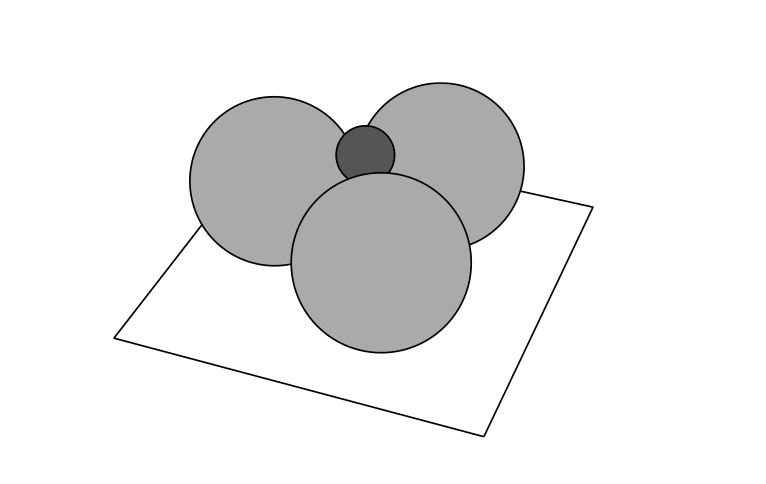
\includegraphics[width=1\textwidth]{ЭлМШ 2025-2026/III блок/10/Тренировки/II/Решения/11.5.png}
\end{center}

\newpage

\hspace{3mm}

\textit{Решение.} Центры волейбольных мячей обозначим через $A, B, C$, а центр теннисного через $D$; верхнюю точку теннисного мяча обозначим через $X$.

Рассмотрим сечение волейбольных мячей плоскостью $A B C$ (рис. 1). Это три попарно касающиеся окружности радиусом 18 . Следовательно, точки $A, B, C$ расположены в вершинах правильного треугольника со стороной 36 . Центр этого треугольника обозначим за $O$; тогда $O A=18 / \cos \left(30^{\circ}\right)=12 \sqrt{3}$ (из прямоугольного треугольника $O A M$, где $M$ - середина $A B$ ).

\begin{figure}[h]
    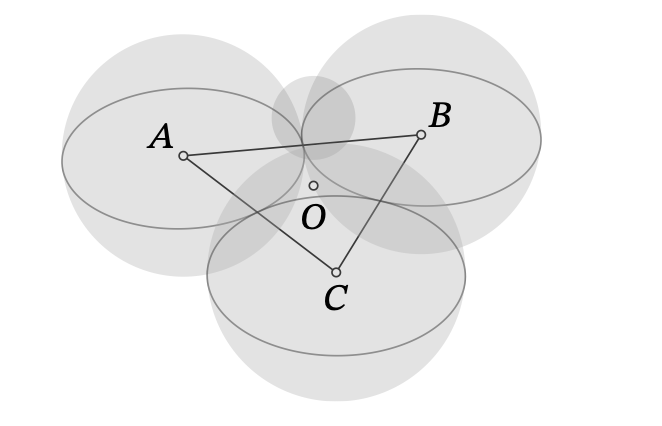
\includegraphics[width=0.4\linewidth]{ЭлМШ 2025-2026/III блок/10/Тренировки/II/Решения/11.5.1.png}
    \caption{}
    \label{fig:placeholder}
\end{figure}


Из соображений симметрии ясно, что точки $X, D$ и $O$ лежат на одной вертикальной прямой. Рассмотрим сечение теннисного мяча и одного из волейбольных плоскостью $A D O$ (рис. 2). Треугольник $A D O$ прямоугольный, $A D=18+6=24$, по теореме Пифагора имеем

$$
O D=\sqrt{A D^2-O A^2}=12 .
$$

\begin{figure}[h]
    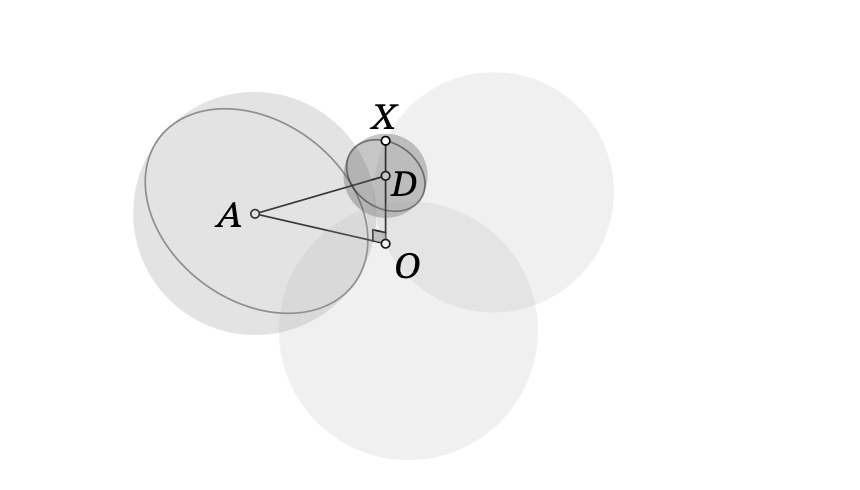
\includegraphics[width=0.5\linewidth]{image.png}
    \caption{}
    \label{fig:placeholder}
\end{figure}

\newpage

\hspace{3mm}

Сама точка $O$, как и вся плоскость $A B C$, находится на высоте радиуса волейбольного мяча, то есть 18 ; точка $D$, как мы выяснили, выше неё на 12 ; а точка $X$ выше точки $D$ на радиус теннисного мяча, то есть на 6 . В сумме получаем $18+12+6=36$.
%11.5 Москва 2022
